\documentclass[a4paper,12pt]{article} % This defines the style of your paper

\usepackage[top = 2.5cm, bottom = 2.5cm, left = 2.5cm, right = 2.5cm]{geometry} 

% Unfortunately, LaTeX has a hard time interpreting German Umlaute. The following two lines and packages should help. If it doesn't work for you please let me know.
\usepackage[T1]{fontenc}
\usepackage[utf8]{inputenc}
\usepackage{subcaption}

% The following two packages - multirow and booktabs - are needed to create nice looking tables.
\usepackage{multirow} % Multirow is for tables with multiple rows within one cell.
\usepackage{booktabs} % For even nicer tables.
\usepackage{amsmath}
\usepackage{bm}

% As we usually want to include some plots (.pdf files) we need a package for that.
\usepackage{graphicx} 
\usepackage{rotating}
\usepackage{cancel}

% The default setting of LaTeX is to indent new paragraphs. This is useful for articles. But not really nice for homework problem sets. The following command sets the indent to 0.
\usepackage{setspace}
\setlength{\parindent}{0in}

% Package to place figures where you want them.
\usepackage{float}

% The fancyhdr package let's us create nice headers.
\usepackage{fancyhdr}

\usepackage[utf8]{inputenc}
\usepackage[portuguese]{babel}
\usepackage{makecell}
\usepackage{listings}
\usepackage{xcolor}

\definecolor{codegreen}{rgb}{0,0.6,0}
\definecolor{codegray}{rgb}{0.5,0.5,0.5}
\definecolor{codepurple}{rgb}{0.58,0,0.82}
\definecolor{backcolour}{rgb}{0.95,0.95,0.92}

\lstdefinestyle{mystyle}{
    backgroundcolor=\color{backcolour},   
    commentstyle=\color{codegreen},
    keywordstyle=\color{magenta},
    numberstyle=\tiny\color{codegray},
    stringstyle=\color{codepurple},
    basicstyle=\ttfamily\footnotesize,
    breakatwhitespace=false,         
    breaklines=true,                 
    captionpos=b,                    
    keepspaces=true,                 
    numbers=left,                    
    numbersep=5pt,                  
    showspaces=false,                
    showstringspaces=false,
    showtabs=false,                  
    tabsize=2
}
\lstset{style=mystyle}
\renewcommand{\arraystretch}{1.5}

\pagestyle{fancy} % With this command we can customize the header style.

\fancyhf{} % This makes sure we do not have other information in our header or footer.

\lhead{\footnotesize Homework 4}% \lhead puts text in the top left corner. \footnotesize sets our font to a smaller size.

%\rhead works just like \lhead (you can also use \chead)
\rhead{\footnotesize Joana Pimenta, Rodrigo Laia} %<---- Fill in your lastnames.

% Similar commands work for the footer (\lfoot, \cfoot and \rfoot).
% We want to put our page number in the center.
\cfoot{\footnotesize \thepage} 

\begin{document}

\thispagestyle{empty} % This command disables the header on the first page. 

\begin{tabular}{p{15.5cm}} % This is a simple tabular environment to align your text nicely 
{\large \bf Aprendizagem} \\
Instituto Superior Técnico \\ outubro  de 2023  \\ \\ 
\hline % \hline produces horizontal lines.
\\
\end{tabular} % Our tabular environment ends here.

\vspace*{0.3cm} % Now we want to add some vertical space in between the line and our title.

\begin{center} % Everything within the center environment is centered.
	{\Large \bf Homework 4 - Report} % <---- Don't forget to put in the right number
	\vspace{2mm}
	
        % YOUR NAMES GO HERE
	{\bf Joana Pimenta (103730), Rodrigo Laia (102674) } % <---- Fill in your names here!
		
\end{center}  

\vspace{0.4cm}

\section*{Pen and Paper}
\begin{enumerate}

\item Fórmulas utilizadas:

\begin{equation}
    \gamma_{ki} = p(c_k|\mathbf{x}_i) = \frac{p(c_k)p(\mathbf{x}_i|c_k)}{p(\mathbf{x}_i)}
\end{equation}

\begin{equation}
    p(\mathbf{x}_i) = p(c_1)p(\mathbf{x}_i|c_1)+p(c_2)p(\mathbf{x}_i|c_2)
\end{equation}

\begin{equation}
    p(\mathbf{x}_i|c_k) =
    \begin{cases} 
        p_{k} \cdot \mathcal{N}(\mathbf{x}_i|\boldsymbol{\mu}_k,\boldsymbol{\Sigma}_k) & \text{se } y_1 = 1 \\
        (1-p_k) \cdot \mathcal{N}(\mathbf{x}_i|\boldsymbol{\mu}_k,\boldsymbol{\Sigma}_k) & \text{se } y_1 = 0 
    \end{cases}
\end{equation}

\textbf{E-step:} \\ \\

Cálculo das probabilidades $p(\textbf{x}_i)$
\begin{equation*}
    p(\textbf{x}_1) = 0.05185
\end{equation*}

\begin{equation*}
    p(\textbf{x}_2) = 0.02775
\end{equation*}

\begin{equation*}
    p(\textbf{x}_3) = 0.04337
\end{equation*}

\begin{equation*}
    p(\textbf{x}_4) = 0.05243
\end{equation*}

Cálculos dos $\gamma_{ki}$

\begin{equation*}
    \gamma_{k=1,i=1} = 0.19259
\end{equation*}

\begin{equation*}
    \gamma_{k=2,i=1} = 0.80741
\end{equation*}

\begin{equation*}
    \gamma_{k=1,i=2} = 0.63135
\end{equation*}

\begin{equation*}
    \gamma_{k=2,i=2} = 0.36865
\end{equation*}

\begin{equation*}
    \gamma_{k=1,i=3} = 0.55181
\end{equation*}

\begin{equation*}
    \gamma_{k=2,i=3} = 0.44819
\end{equation*}

\begin{equation*}
    \gamma_{k=1,i=4} = 0.16892
\end{equation*}

\begin{equation*}
    \gamma_{k=2,i=4} = 0.83108
\end{equation*}

\textbf{M-step:} \\ \\
Cada observação $\mathbf{x}_i$ permite atualizar os parâmetros com peso $\gamma_{ki}$. 
Assim calculamos os novos parâmetros atualizados para cada cluster utilizando as seguintes fórmulas. 

\begin{equation}
    N_k = \sum_{i=1}^4 \gamma_{ki}
\end{equation}

\begin{equation}
    \pi_k = \frac{N_k}{N}
\end{equation}
% o parâmetro de uma distribuição de Bernoulli é a probabilidade de sucesso, 
% ou seja, a probabilidade de a y_1 assumir o valor 1.
% Ela é dada pelo numero total de observações em que y_1 é 1 dividido pelo numero total de observações
% no entanto, neste caso cada observação tem um peso diferente, dado pelo gamma_ki
% assim, o parâmetro da distribuição de Bernoulli é dado por:
\begin{equation}
    P_k(y_1=1) = \frac{\sum_{i=1}^4 \gamma_{ki} \cdot p(y_1=1|\mathbf{x}_i)}{\sum_{i=1}^4 \gamma_{ki}} 
\end{equation}
Nota: A probabilidade $p(y_1=1|\mathbf{x}_i)$ é 1 se $y_1$ de $\mathbf{x}_i$ for 1 e 0 caso contrário. 

\begin{equation}
    \boldsymbol{\mu}_k = \frac{1}{N_k} \sum_{i=1}^4 \gamma_{ki} \mathbf{x}_i    
\end{equation}

\begin{equation}
    \boldsymbol{\Sigma}_k = \frac{1}{N_k} \sum_{i=1}^4 \gamma_{ki} (\mathbf{x}_i - \boldsymbol{\mu}_k)(\mathbf{x}_i - \boldsymbol{\mu}_k)^T
\end{equation}


Parâmetros atualizados:

\begin{equation*}
    \pi_1 = 0.38617
\end{equation*}

\begin{equation*}
    \pi_2 = 0.61383
\end{equation*}

\begin{equation*}
    P_{k=1}(y_1=1) = 0.23404
\end{equation*}

\begin{equation*}
    P_{k=2}(y_1=1) = 0.66732
\end{equation*}

\begin{equation*}
    \boldsymbol{\mu}_1 = \begin{bmatrix}
    0.02651 \\
    0.50713
\end{bmatrix}
\end{equation*}

\begin{equation*}
    \boldsymbol{\mu}_2 = \begin{bmatrix}
    0.30914 \\
    0.21042
\end{bmatrix}
\end{equation*}

\begin{equation*}
    \boldsymbol{\Sigma}_1 = \begin{bmatrix}
    0.14137 & -0.10541 \\
    -0.10541 & 0.09605
\end{bmatrix}
\end{equation*}

\begin{equation*}
    \boldsymbol{\Sigma}_2 = \begin{bmatrix}
    0.10829 & -0.08865 \\
    -0.08865 & 0.10412
\end{bmatrix}
\end{equation*}

\item
Para calcular os posteriors da observação $\mathbf{x}_{new}$ utilizamos a 
seguinte fórmula:

\begin{equation}
    p(cluster = k|\mathbf{x}_{new}) = \frac{p(cluster = k)p(\mathbf{x}_{new}|cluster = k)}{p(\mathbf{x}_{new})}
\end{equation}

Em que $p(cluster = k)$ é dado por $\pi_k$ e $p(\mathbf{x}_{new}|cluster = k)$ é dado pela fórmula (3).

Cálculos:

\begin{equation*}
    p(\mathbf{x}_{new}) = 0.03048
\end{equation*}

\begin{equation*}
    p(cluster = 1|\mathbf{x}_{new}) = 0.08029
\end{equation*}

\begin{equation*}
    p(cluster = 2|\mathbf{x}_{new}) = 0.91971
\end{equation*}

Assim conclui-se que a observação $\mathbf{x}_{new}$ pertence ao cluster 2 com probabilidade 0.91971
e ao cluster 1 com probabilidade 0.08029.

\item Neste exercício assumimos que o cluster atribuído a cada observação é 
é escolhido pelo critério de \textit{maximum likelihood}.
Assim, o cluster escolhido é dado por:

\begin{equation}
    cluster = \arg\max_k p(\mathbf{x}_i|cluster = k)
\end{equation}

Em que $p(\mathbf{x}_i|cluster = k)$ é dado pela fórmula (3). \\ \\

Assim,

\begin{table}[H]
\centering
\begin{tabular}{|c|c|c|c|}
\hline
Observação & $p(\mathbf{x}_i|cluster = 1)$ & $p(\mathbf{x}_i|cluster = 2)$ & Cluster atribuído\\ \hline
$\mathbf{x_1}$ &  0.23147  & 0.94954 & 2 \\ \hline
$\mathbf{x_2}$ &  1.26633  & 0.08874 & 1 \\ \hline
$\mathbf{x_3}$ &  1.43811  & 0.45417 & 1 \\ \hline
$\mathbf{x_4}$ &  0.02077  & 0.72331 & 2 \\ \hline
\end{tabular}
\end{table}

Coeficiente de Silhueta:

\begin{equation}
    s_i = 1 - \frac{a(\mathbf{x}_i)}{b(\mathbf{x}_i)}
\end{equation}

em que $a(\mathbf{x}_i)$ é a distância média entre $\mathbf{x}_i$ e as outras 
observações no mesmo cluster e $b(\mathbf{x}_i)$ é a distância média entre 
$\mathbf{x}_i$ e as observações no outro cluster. \\ \\

A silhueta de um cluster é dada pela média dos coeficientes de silhueta de todas
as observações pertencentes a esse cluster. \\ \\

A silhueta da solução é por sua vez dada pela média das silhuetas de todos os
clusters. \\ \\

Neste caso a distância considerada é a distância de Manhattan, logo:

\begin{equation}
    d(\mathbf{u},\mathbf{v}) = \sum_{i=1}^n |u_i - v_i|
\end{equation}

Assim, as silhuetas obtidas foram:

\begin{table}[H]
\centering
\begin{tabular}{|c|c|c|c|c|c|c|}
\hline
cluster           & $\mathbf{x}_i$ & a$(\mathbf{x}_i)$ & b$(\mathbf{x}_i)$ & s$(\mathbf{x}_i)$  & s(cluster)& s(sol)\\ \hline
\multirow{2}{*}{1} & $\mathbf{x}_2$ & 0.9 & 2.7 & 0.(6)  & \multirow{2}{*}{0.58(3)} & \multirow{4}{*}{0.702(7)} \\ \cline{2-5}
                    & $\mathbf{x}_3$ & 0.9 & 1.7(9) & 0.4(9) & &  \\ \cline{1-6}
\multirow{2}{*}{2} & $\mathbf{x}_1$ & 0.3(9) & 2.25 &0.8(2) & \multirow{2}{*}{0.8(2)}  & \\ \cline{2-5}
                    & $\mathbf{x}_4$ & 0.3(9) & 2.25 & 0.8(2) &  &   \\ \hline
\end{tabular}
\end{table}
\item 

A purity é dada por:

\begin{equation}
    \text{purity} = \frac{1}{N} \sum_{k=1}^K \max_j |c_k \cap t_j| = \frac{1}{N} \left( \max_j |c_1 \cap t_j| + \max_j |c_2 \cap t_j| \right)
\end{equation}


Uma vez que temos uma purity de 0.75 e um número total de observações de 4,
então $\frac{1}{N} \left( \max_j |c_1 \cap t_j| + \max_j |c_2 \cap t_j| \right) = 0.75 \times 4 = 3$ \\ \\

Logo podemos ter os seguintes casos:
\begin{enumerate}
    \item $\max_j |c_1 \cap t_j| = 3$ e $\max_j |c_2 \cap t_j| = 0$
    \item $\max_j |c_1 \cap t_j| = 2$ e $\max_j |c_2 \cap t_j| = 1$
    \item $\max_j |c_1 \cap t_j| = 1$ e $\max_j |c_2 \cap t_j| = 2$
    \item $\max_j |c_1 \cap t_j| = 0$ e $\max_j |c_2 \cap t_j| = 3$
\end{enumerate}

As opções (a) e (d) não são possíveis porque os clusters 2 e 1 só têm 2 observações cada um. 

\textbf{Opção (b)} \\ 
Neste caso, as observações do cluster 1 são as duas classificadas corretamente. 
No cluster 2 uma é corretamente identificada e a outra não. Assim, as observações 
no cluster 1 têm a mesma classificação; uma das observações do cluster 2 tem classificação
diferente das do cluster 1 e a outra pode ter classificação igual às do cluster 1 (opção 1)
ou diferente, sendo que neste caso é também diferente da classificação do outra observação
do cluster 2 (opção 2). Assim, conclui-se que o número verdadeiro de classes pode ser 2 ou 3. \\
Para visualizar melhor as opções possíveis fizemos os seguintes esquemas 
(bolas de cores diferentes representam classes verdadeiras diferentes):

\begin{figure}[H]
\centering
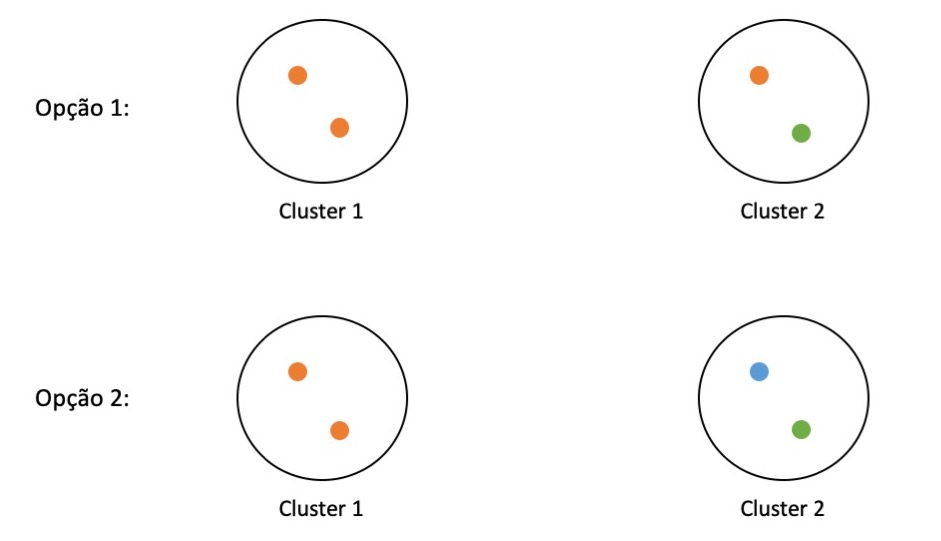
\includegraphics[width=0.7\textwidth]{ex4_clusters.jpg}
\end{figure}

\textbf{Opção (c)} \\
O raciocínio é semelhante ao da opção (b). Conclui-se que o número verdadeiro de classes pode ser 2 ou 3.

\end{enumerate}

\clearpage

\section*{Programming - Código Python e Resultados Obtidos}

\begin{enumerate}

\item 
Código Utilizado:

\begin{lstlisting}[language=Python]

\end{lstlisting}

\item 

Código Utilizado:

\begin{lstlisting}[language=Python]

\end{lstlisting}

\item

Código Utilizado:

\begin{lstlisting}[language=Python]

\end{lstlisting}

\item 
\end{enumerate}

\end{document}
